\documentclass{article}
        \usepackage[utf8]{inputenc}
        \usepackage{tikz}
        \usepackage{xcolor}
        \usepackage{graphicx}
        \usepackage{amsmath}
        \usepackage{caption}

        \definecolor{brightmaroon}{RGB}{195,33,72}
        \definecolor{cyan}{RGB}{0,255,255}
        \definecolor{skyblue}{RGB}{135,206,235}

        \begin{document}
        \begin{figure}[htbp]
        \centering
        \resizebox{.45\linewidth}{!}{
        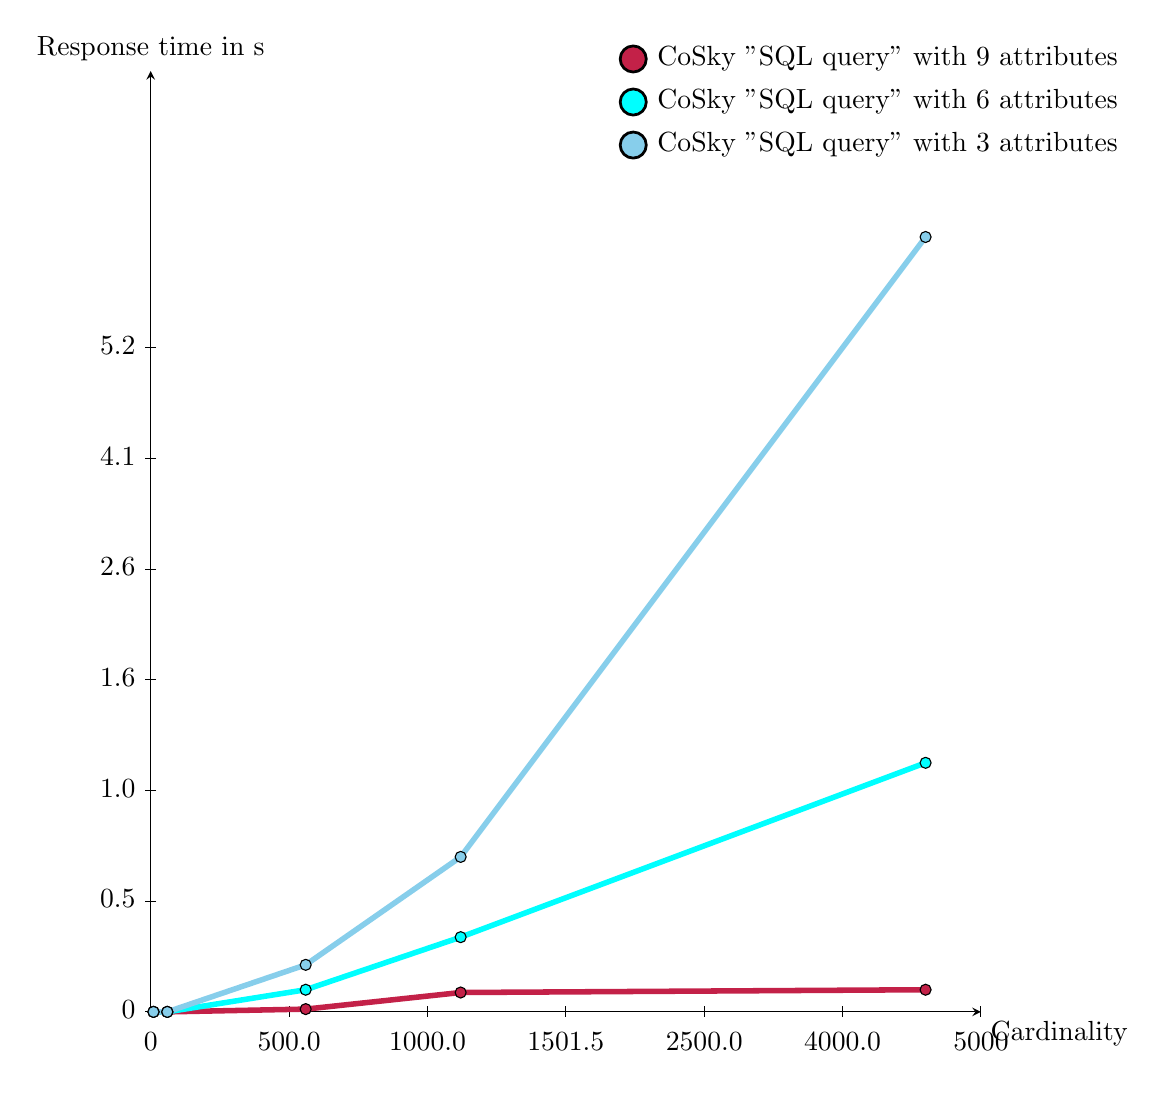
\begin{tikzpicture}[line join=bevel,
        biggraynode/.style={shape=circle, fill=gray, draw=black, line width=1pt},
        bigbrightmaroonnode/.style={shape=circle, fill=brightmaroon, draw=black, line width=1pt},
        bigcyannode/.style={shape=circle, fill=cyan, draw=black, line width=1pt},
        bigskybluenode/.style={shape=circle, fill=skyblue, draw=black, line width=1pt}]
        \draw[-stealth] (0pt, 0pt) -- (300pt, 0pt) node[anchor=north west] {Cardinality};
        \draw[-stealth] (0pt, 0pt) -- (0pt, 340pt) node[anchor=south] {Response time in s};
        % X-axis ticks and labels
                \foreach \x/\xtext in {0pt/$0$, 50pt/$500.0$, 100pt/$1000.0$, 150pt/$1501.5$, 200pt/$2500.0$, 250pt/$4000.0$, 300pt/$5000$} {
                  \draw (\x, 2pt) -- (\x, -2pt) node[below] {\xtext\strut};
                }
                % Y-axis ticks and labels
                \foreach \y/\ytext in {0pt/$0$, 40pt/$0.5$, 80pt/$1.0$, 120pt/$1.6$, 160pt/$2.6$, 200pt/$4.1$, 240pt/$5.2$} {
                  \draw (2pt, \y) -- (-2pt, \y) node[left] {\ytext\strut};
                }
                % Lines
\draw[brightmaroon, line width=2pt](1pt, 0pt) -- (6pt, 0pt) -- (56pt, 1pt) -- (112pt, 7pt) -- (280pt, 8pt);
\draw[cyan, line width=2pt](1pt, 0pt) -- (6pt, 0pt) -- (56pt, 8pt) -- (112pt, 27pt) -- (280pt, 90pt);
\draw[skyblue, line width=2pt](1pt, 0pt) -- (6pt, 0pt) -- (56pt, 17pt) -- (112pt, 56pt) -- (280pt, 280pt);
% Points and labels
\filldraw[color=black, fill=brightmaroon] (1pt, 0pt) circle (2pt);
\filldraw[color=black, fill=brightmaroon] (6pt, 0pt) circle (2pt);
\filldraw[color=black, fill=brightmaroon] (56pt, 1pt) circle (2pt);
\filldraw[color=black, fill=brightmaroon] (112pt, 7pt) circle (2pt);
\filldraw[color=black, fill=brightmaroon] (280pt, 8pt) circle (2pt);
\filldraw[color=black, fill=cyan] (1pt, 0pt) circle (2pt);
\filldraw[color=black, fill=cyan] (6pt, 0pt) circle (2pt);
\filldraw[color=black, fill=cyan] (56pt, 8pt) circle (2pt);
\filldraw[color=black, fill=cyan] (112pt, 27pt) circle (2pt);
\filldraw[color=black, fill=cyan] (280pt, 90pt) circle (2pt);
\filldraw[color=black, fill=skyblue] (1pt, 0pt) circle (2pt);
\filldraw[color=black, fill=skyblue] (6pt, 0pt) circle (2pt);
\filldraw[color=black, fill=skyblue] (56pt, 17pt) circle (2pt);
\filldraw[color=black, fill=skyblue] (112pt, 56pt) circle (2pt);
\filldraw[color=black, fill=skyblue] (280pt, 280pt) circle (2pt);
%% Caption
        \matrix [below left] at (current bounding box.north east) {
        \node [bigbrightmaroonnode, label=right:CoSky "SQL query" with 9 attributes] {}; \\
        \node [bigcyannode, label=right:CoSky "SQL query" with 6 attributes] {}; \\
        \node [bigskybluenode, label=right:CoSky "SQL query" with 3 attributes] {}; \\
        };
        \end{tikzpicture}
        }
        \caption{CoSky response time for SQL queries}
        \label{fig:temps_de_reponse_de_CoSky_en_sql}
        \end{figure}
        \end{document}